\documentclass[12pt]{article}

\usepackage[portuguese]{babel}
\usepackage[utf8]{inputenc}
\usepackage{amsmath}
\usepackage{commath}
\usepackage{booktabs}
\usepackage[alf]{abntex2cite}
\usepackage{indentfirst}
\usepackage{graphicx}
\usepackage{multicol,lipsum}
\usepackage{geometry}
\usepackage[alf]{abntex2cite}
\usepackage{subfigure}
\graphicspath{{../../Figures/Report_19_09/}{../../Images/Report_19_09/}}

\geometry{
  paper = a4paper,
  inner = 3cm,
  outer = 3cm,
  top = 2cm,
  bottom = 2cm
}

\begin{document}
%\maketitle

\onehalfspacing

\begin{titlepage}
\begin{center}

\Huge{Universidade Federal de Alagoas}\\
\large{Instituto de Computação}\\ 
\large{Laboratório de Computação Científica e Análise Numérica}\\ 
\vspace{220pt}
\textbf{\LARGE{Research report}}\\
%\title{{\large{Título}}}
\vspace{3,5cm}
\end{center}

\begin{flushleft}
\begin{tabbing}
Student: Danilo Fernandes Costa\\
Professor: Alejandro Frery\\
\end{tabbing}
\end{flushleft}
\vspace{1cm}

\begin{center}
\vspace{\fill}
September\\
2019
\end{center}
\end{titlepage}

\section{Introduction}

In this report, some results of the analysis of samples referring to plantation regions observed over time are shown. The first observation was made on 16 May 2016, which was followed by four others with a time interval of 24 days between adjacent observations. 
Those regions consist of three soybeans crops, three wheat, two oats and two canola and are shown in the figures \ref{fig:r1} to \ref{fig:r5}. Those samples were obtained using the classification of the regions given in the figure \ref{fig:classes}.

The results consist of the graphic adjusting of the beta distribution to the histograms of the distances of the samples to the trihedral and random volume scatterers. In addition, the Kolmogorov-Smirnov good-of-fit test was performed to validate the hypothesis of the adjust. The choice of these scatterers is because they were more sensitive to vegetation variation in the analyzed regions, which can be verified in the figures \ref{fig:tp} and \ref{fig:rvp} that contain respectively the pixel proportions in the sample that is more similar to trihedral and the random volume as a function of time.

\begin{figure}[!h]
\centering
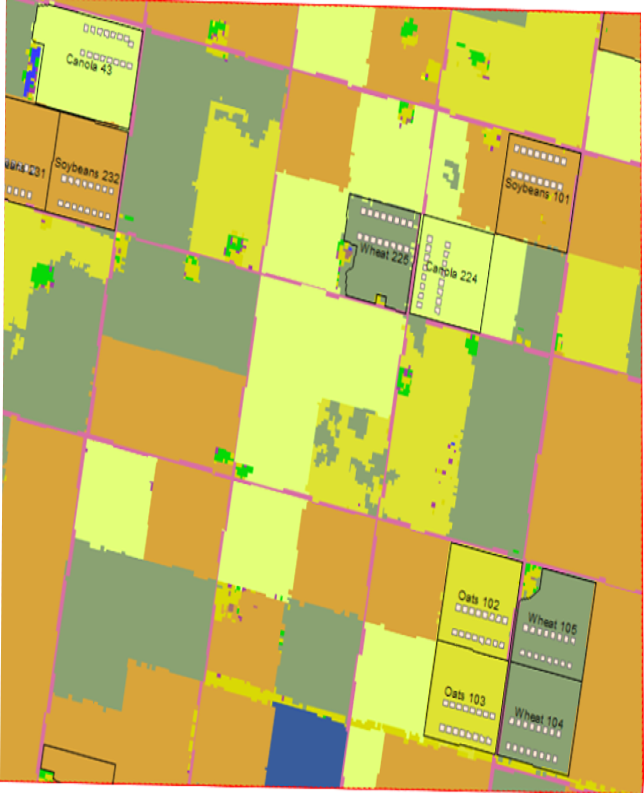
\includegraphics[width = .55\linewidth]{/Regions/classes}
\label{fig:classes}
\caption{Classification of the regions on the PolSAR image}
\end{figure}

\begin{figure*}[!h]
\centering

\subfigure[1th observation\label{fig:r1}]{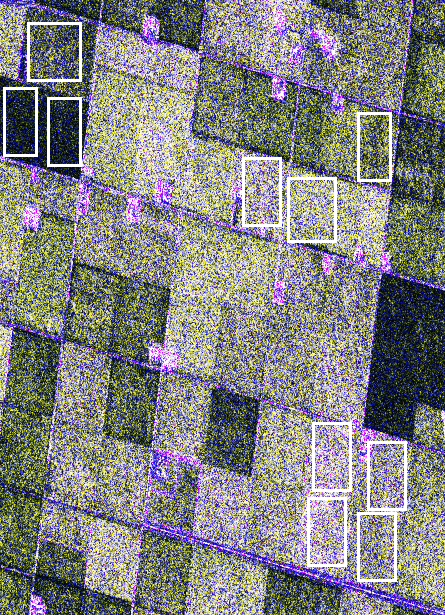
\includegraphics[width = .32\linewidth]{/Regions/regions_1}}
\subfigure[2th observation\label{fig:r2}]{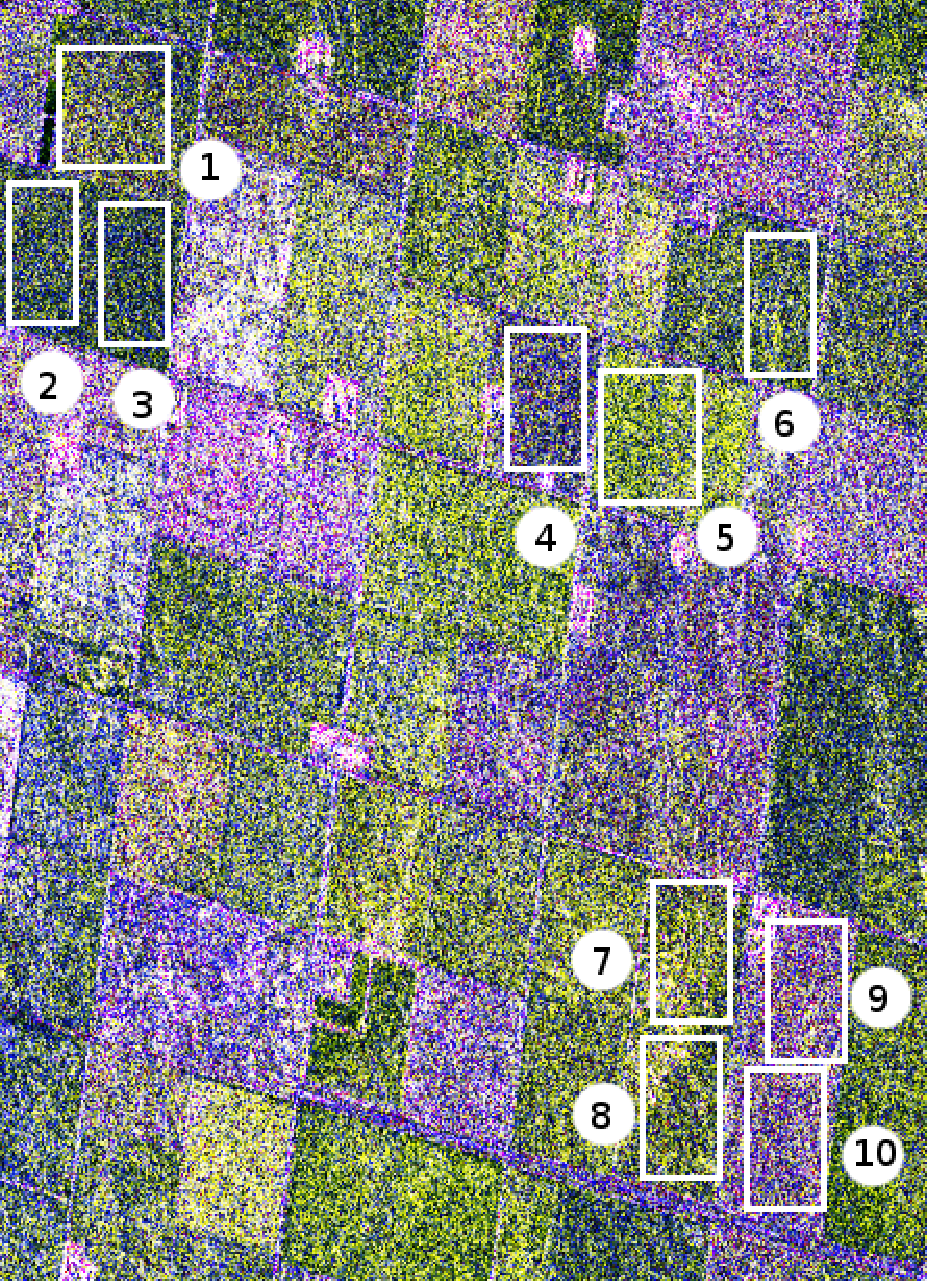
\includegraphics[width = .32\linewidth]{/Regions/regions_2}}
\subfigure[3th observation\label{fig:r3}]{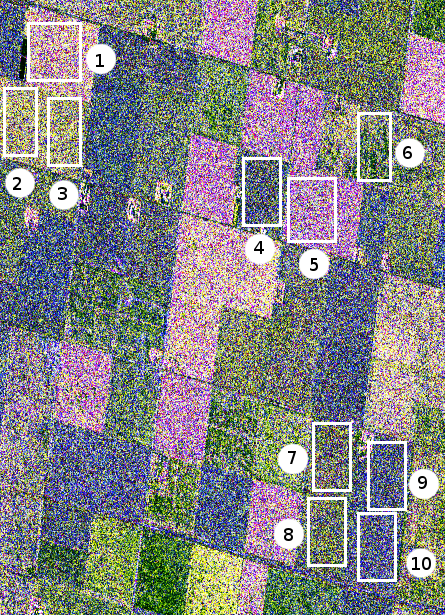
\includegraphics[width = .32\linewidth]{/Regions/regions_3}}
\subfigure[4th observation\label{fig:r4}]{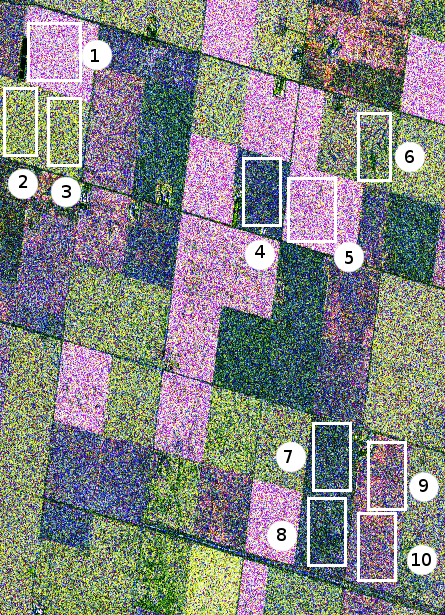
\includegraphics[width = .32\linewidth]{/Regions/regions_4}}
\subfigure[5th observation\label{fig:r5}]{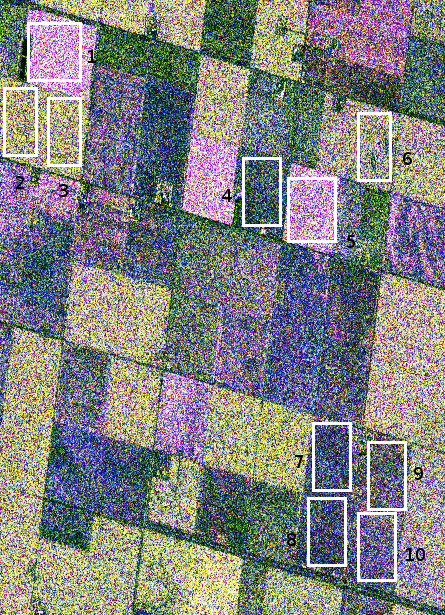
\includegraphics[width = .32\linewidth]{/Regions/regions_5}}

\caption{Samples analysed over time in where 1 to 10 corresponding respectively to Canola 43, Soybeans 231, Soybeans 232, Wheat 225, Canola 224, Soybeans 101, Oats 102, Oats 103, Wheat 105 and Wheat 104}
\label{fig:regions}
\end{figure*}

\begin{figure*}[!h]
\centering
\subfigure[Trihedral\label{fig:tp}]{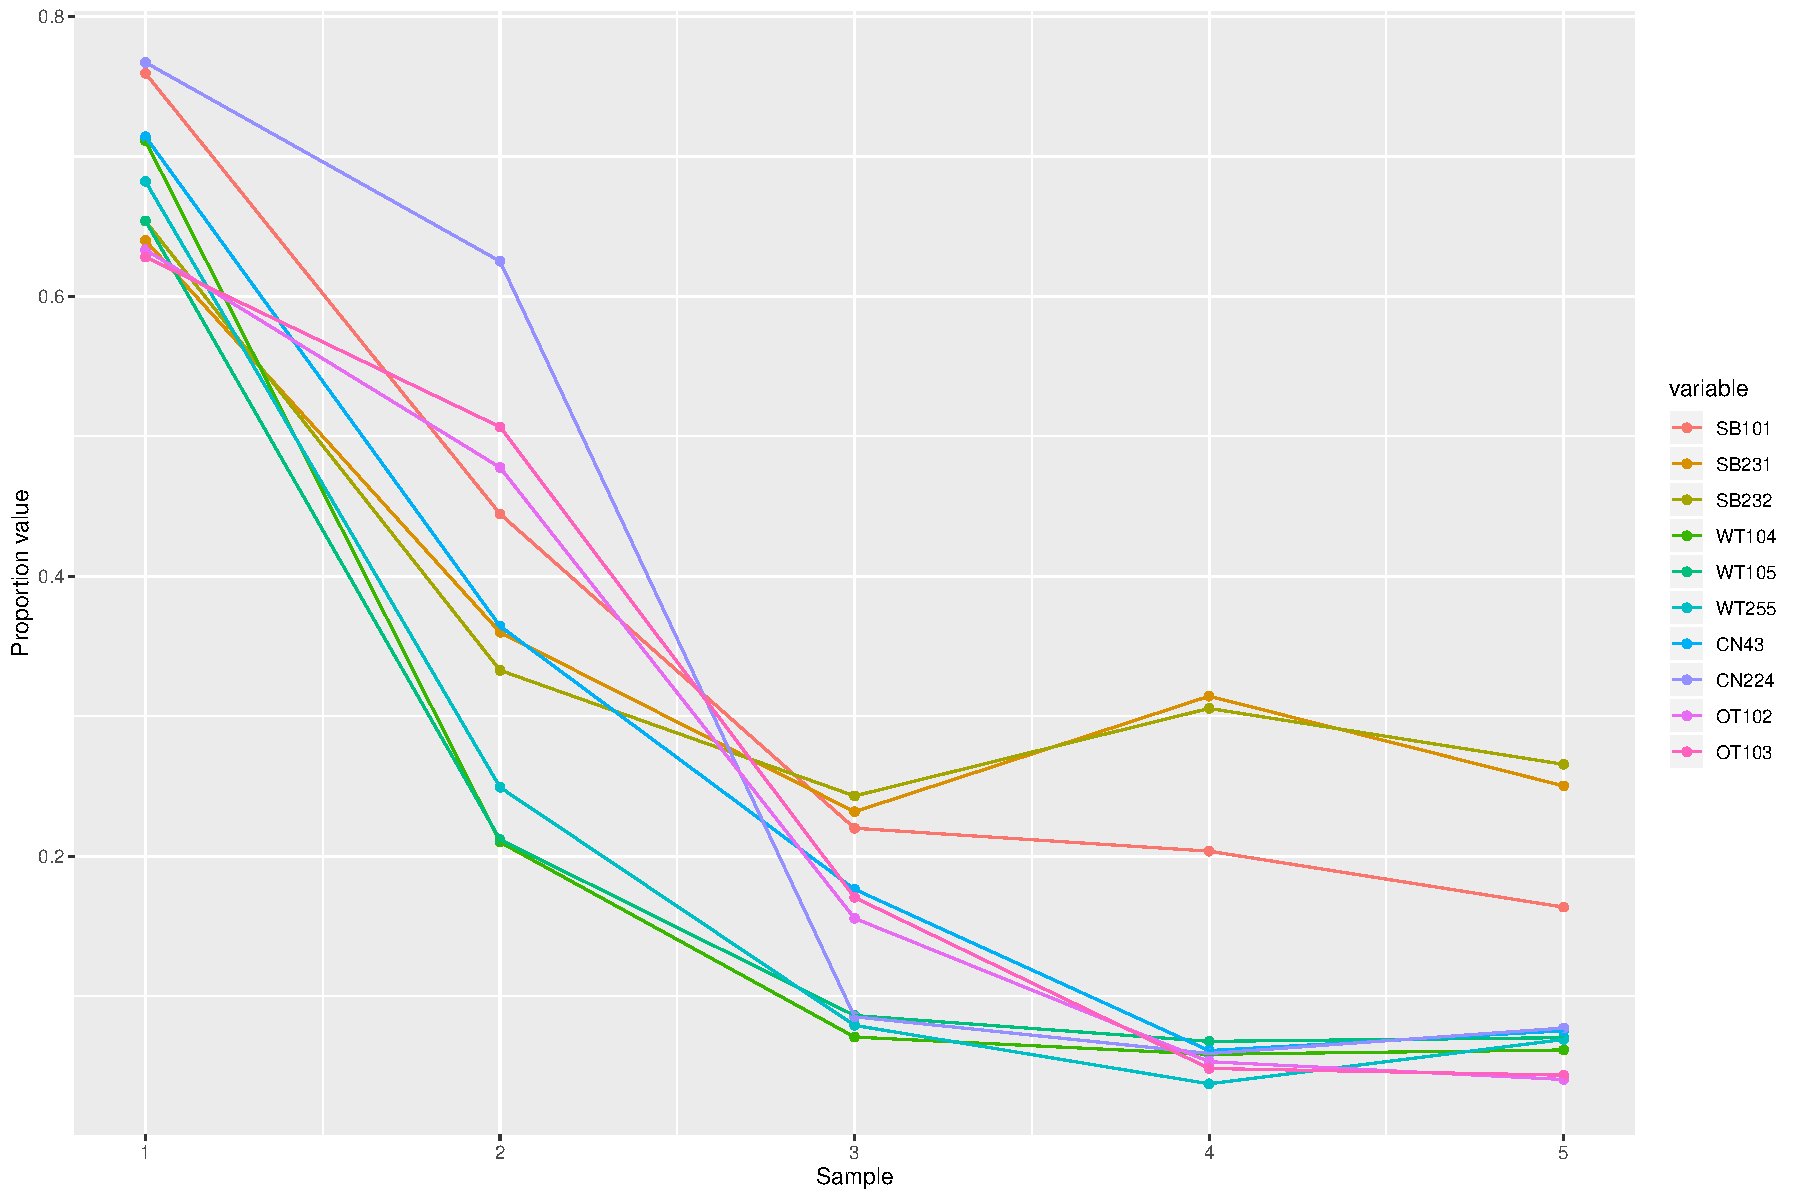
\includegraphics[width = .49\linewidth]{/Parameters/tri_proportion}}
\subfigure[Random Volume\label{fig:rvp}]{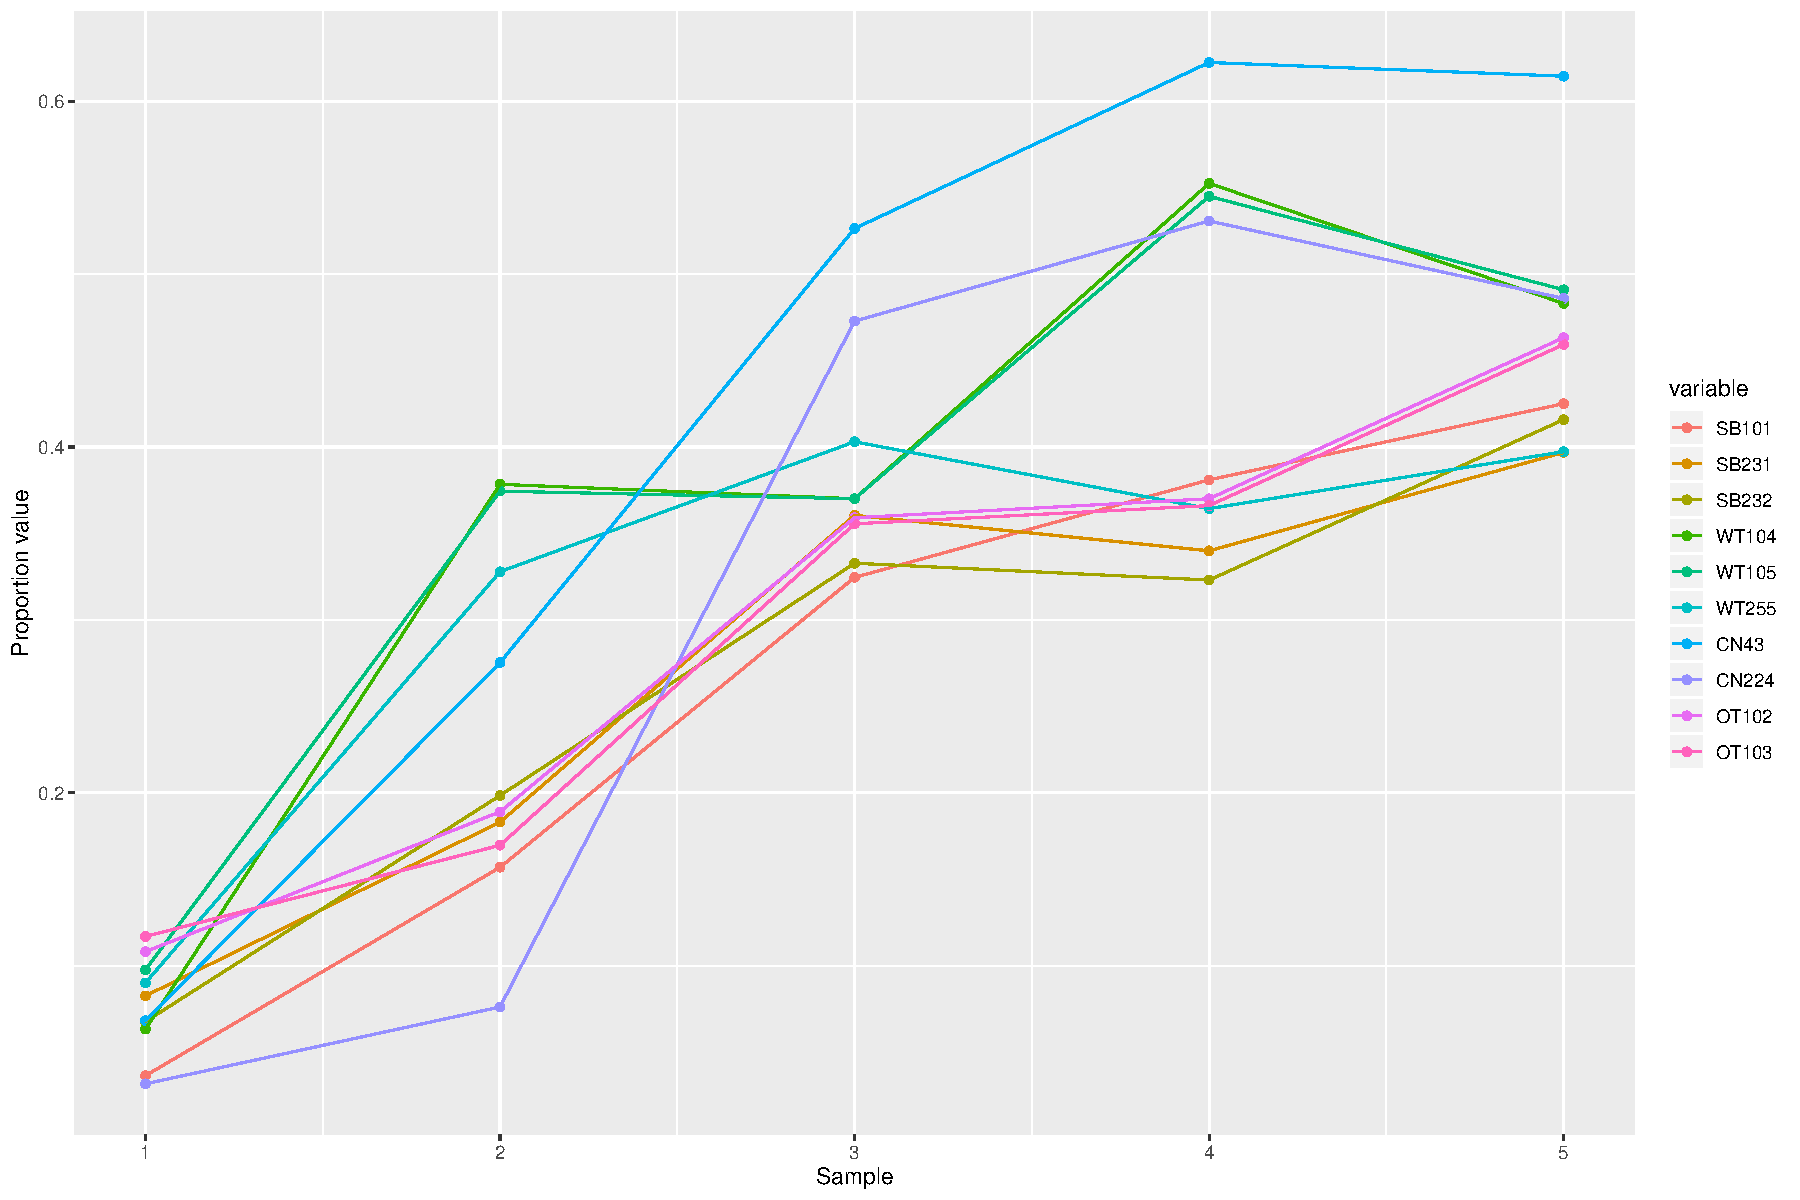
\includegraphics[width = .49\linewidth]{/Parameters/rv_proportion}}
\caption{Pixel proportions on the analysed regions more similar to trihedral and random volume as function of time, where SB, WT, CN and OT indicate respectively Soybeans, Wheat, Canola and Oats}
\label{fig:pixel_proportions}
\end{figure*}

\newpage

\section{Adjust the histograms to the Beta Distribution}

The figures \ref{fig:sb101_hist_tri} to \ref{fig:ot103_hist_rv} contain the histograms of the Geodesic Distances between the scatterer (random or trihedral volume) and the pixels of the sample most similar to this scatterer.
The number of those pixels are in the table \ref{tab:size_sample} which TR and RV indicates respectively trihedral and random volume. In addiction, the histograms are graphically adjusted by the Beta Distribution, whose parameters were estimated from the distances analyzed.

Those adjusts was verified by Komolgorov-Smirnov good-of-fit test whose obtained $p$-values are in the table \ref{tab:pvalues_table}. In this table, the biggest and least $p$-values are in bold.

\begin{table}[hbt]
\centering
\caption{Number of pixels more similar to trihedral and random volume}\label{tab:size_sample}
\begin{tabular}{lrrrrrrrrrr}

\toprule
& \multicolumn{2}{c}{First} & \multicolumn{2}{c}{Second} & \multicolumn{2}{c}{Third} & \multicolumn{2}{c}{Fourth} & \multicolumn{2}{c}{Fifth}\\
& \multicolumn{2}{c}{observation} & \multicolumn{2}{c}{observation} & \multicolumn{2}{c}{observation} & \multicolumn{2}{c}{observation} & \multicolumn{2}{c}{observation}\\
& TR & RV & TR & RV & TR & RV & TR & RV& TR & RV\\
\cmidrule(lr){2-11}
\textbf{SB 101} & 1481 & 71 & 867 & 306 & 429 & 633 & 397 & 743 & 319 & 829\\
\textbf{SB 231} & 1285 & 148 & 656 & 381 & 449 & 706 & 615 & 649 & 508 & 775\\
\textbf{SB 232} & 1275 & 132 & 649 & 387 & 474 & 649 & 596 & 630 & 518 & 811\\
\textbf{WT 104} & 1618 & 144 & 478 & 861 & 161 & 842 & 133 & 1257 & 140 & 1099\\
\textbf{WT 105} & 1488 & 222 & 482 & 852 & 196 & 842 & 154 & 1240 & 160 & 1117\\
\textbf{WT 255} & 1552 & 205 & 567 & 746 & 180 & 917 & 85 & 829 & 157 & 904\\
\textbf{CN 43}  & 1964 & 155 & 1002 & 625 & 485 & 1195 & 168 & 1413 & 207 & 1395\\
\textbf{CN 224} & 2106 & 87 & 1716 & 209 & 234 & 1298 & 162 & 1457 & 212 & 1334\\
\textbf{OT 102} & 1441 & 246 & 1087 & 430 & 354 & 817 & 121 & 842 & 92 & 1054\\
\textbf{OT 103} & 1429 & 266 & 1153 & 386 & 388 & 806 & 110 & 833 & 99 & 1045\\
\bottomrule
\end{tabular} 
\end{table}


\begin{table}[hbt]
\centering
\caption{$p$-values of the Kolmogorov-Smirnov goodness-of-fit test of the distances to trihedral an random volume}\label{tab:pvalues_table}
\begin{tabular}{lrrrrrrrrrr}

\toprule
& \multicolumn{2}{c}{First} & \multicolumn{2}{c}{Second} & \multicolumn{2}{c}{Third} & \multicolumn{2}{c}{Fourth} & \multicolumn{2}{c}{Fifth}\\
& \multicolumn{2}{c}{observation} & \multicolumn{2}{c}{observation} & \multicolumn{2}{c}{observation} & \multicolumn{2}{c}{observation} & \multicolumn{2}{c}{observation}\\
& TR & RV & TR & RV & TR & RV & TR & RV& TR & RV\\
\cmidrule(lr){2-11}
\textbf{SB 101} & 0.065 & 0.517 & 0.947 & 0.758 & \textbf{0.059} & 0.495 & 0.452 & 0.109 & 0.401 & 0.144\\
\textbf{SB 231} & 0.775 & 0.242 & 0.573 & 0.166 & 0.314 & 0.275 & 0.239 & 0.114 & 0.416 & 0.070\\
\textbf{SB 232} & 0.244 & 0.340 & 0.968 & 0.328 & 0.713 & 0.070 & 0.422 & 0.357 & 0.163 & 0.630\\
\textbf{WT 104} & 0.178 & 0.715 & 0.421 & 0.094 & 0.514 & 0.779 & 0.062 & 0.369 & 0.602 & 0.919\\
\textbf{WT 105} & 0.231 & 0.090 & 0.069 & 0.139 & 0.557 & 0.613 & 0.108 & 0.195 & 0.192 & 0.252\\
\textbf{WT 255} & 0.235 & 0.513 & 0.270 & 0.375 & 0.628 & 0.279 & 0.653 & 0.069 & 0.437 & \textbf{0.993}\\
\textbf{CN 43}  & 0.238 & 0.406 & 0.217 & 0.202 & 0.930 & 0.318 & 0.623 & 0.732 & 0.262 & 0.747\\
\textbf{CN 224} & 0.184 & 0.116 & 0.128 & 0.333 & 0.298 & 0.714 & 0.813 & 0.409 & 0.305 & 0.391\\
\textbf{OT 102} & 0.289 & 0.191 & 0.243 & 0.532 & 0.384 & 0.212 & 0.710 & 0.370 & 0.928 & 0.396\\
\textbf{OT 103} & 0.096 & 0.139 & 0.139 & 0.186 & 0.265 & 0.079 & 0.936 & 0.079 & 0.989 & 0.489\\
\bottomrule
\end{tabular} 
\end{table}

%SB101
\begin{figure*}[hbt]
\centering
\subfigure[1th observation]{\includegraphics[width = .49\linewidth]{/Histograms/1th_observation/Soybeans_101/histogram_trihedral_1}}
\subfigure[2th observation]{\includegraphics[width = .49\linewidth]{/Histograms/2th_observation/Soybeans_101/histogram_trihedral_2}}
\subfigure[3th observation]{\includegraphics[width = .49\linewidth]{/Histograms/3th_observation/Soybeans_101/histogram_trihedral_3}}
\subfigure[4th observation]{\includegraphics[width = .49\linewidth]{/Histograms/4th_observation/Soybeans_101/histogram_trihedral_4}}
\subfigure[5th observation]{\includegraphics[width = .49\linewidth]{/Histograms/5th_observation/Soybeans_101/histogram_trihedral_5}}
\caption{Histograms of the Geodesic Distances between trihedral and the pixels of the sample extracted from Soybeans 101 most similar to trihedral}
\label{fig:sb101_hist_tri}
\end{figure*}

\begin{figure*}[hbt]
\centering
\subfigure[1th observation]{\includegraphics[width = .49\linewidth]{/Histograms/1th_observation/Soybeans_101/histogram_random_volume_1}}
\subfigure[2th observation]{\includegraphics[width = .49\linewidth]{/Histograms/2th_observation/Soybeans_101/histogram_random_volume_2}}
\subfigure[3th observation]{\includegraphics[width = .49\linewidth]{/Histograms/3th_observation/Soybeans_101/histogram_random_volume_3}}
\subfigure[4th observation]{\includegraphics[width = .49\linewidth]{/Histograms/4th_observation/Soybeans_101/histogram_random_volume_4}}
\subfigure[5th observation]{\includegraphics[width = .49\linewidth]{/Histograms/5th_observation/Soybeans_101/histogram_random_volume_5}}
\caption{Histograms of the Geodesic Distances between random volume and the pixels of the sample extracted from Soybeans 101 most similar to random volume}
\label{fig:sb101_hist_rv}
\end{figure*}

%SB231
\begin{figure*}[hbt]
\centering
\subfigure[1th observation]{\includegraphics[width = .49\linewidth]{/Histograms/1th_observation/Soybeans_231/histogram_trihedral_1}}
\subfigure[2th observation]{\includegraphics[width = .49\linewidth]{/Histograms/2th_observation/Soybeans_231/histogram_trihedral_2}}
\subfigure[3th observation]{\includegraphics[width = .49\linewidth]{/Histograms/3th_observation/Soybeans_231/histogram_trihedral_3}}
\subfigure[4th observation]{\includegraphics[width = .49\linewidth]{/Histograms/4th_observation/Soybeans_231/histogram_trihedral_4}}
\subfigure[5th observation]{\includegraphics[width = .49\linewidth]{/Histograms/5th_observation/Soybeans_231/histogram_trihedral_5}}
\caption{Histograms of the Geodesic Distances between trihedral and the pixels of the sample extracted from Soybeans 231 most similar to trihedral}
\label{fig:sb231_hist_tri}
\end{figure*}

\begin{figure*}[hbt]
\centering
\subfigure[1th observation]{\includegraphics[width = .49\linewidth]{/Histograms/1th_observation/Soybeans_231/histogram_random_volume_1}}
\subfigure[2th observation]{\includegraphics[width = .49\linewidth]{/Histograms/2th_observation/Soybeans_231/histogram_random_volume_2}}
\subfigure[3th observation]{\includegraphics[width = .49\linewidth]{/Histograms/3th_observation/Soybeans_231/histogram_random_volume_3}}
\subfigure[4th observation]{\includegraphics[width = .49\linewidth]{/Histograms/4th_observation/Soybeans_231/histogram_random_volume_4}}
\subfigure[5th observation]{\includegraphics[width = .49\linewidth]{/Histograms/5th_observation/Soybeans_231/histogram_random_volume_5}}
\caption{Histograms of the Geodesic Distances between random volume and the pixels of the sample extracted from Soybeans 231 most similar to random volume}
\label{fig:sb231_hist_rv}
\end{figure*}

%SB232
\begin{figure*}[hbt]
\centering
\subfigure[1th observation]{\includegraphics[width = .49\linewidth]{/Histograms/1th_observation/Soybeans_232/histogram_trihedral_1}}
\subfigure[2th observation]{\includegraphics[width = .49\linewidth]{/Histograms/2th_observation/Soybeans_232/histogram_trihedral_2}}
\subfigure[3th observation]{\includegraphics[width = .49\linewidth]{/Histograms/3th_observation/Soybeans_232/histogram_trihedral_3}}
\subfigure[4th observation]{\includegraphics[width = .49\linewidth]{/Histograms/4th_observation/Soybeans_232/histogram_trihedral_4}}
\subfigure[5th observation]{\includegraphics[width = .49\linewidth]{/Histograms/5th_observation/Soybeans_232/histogram_trihedral_5}}
\caption{Histograms of the Geodesic Distances between trihedral and the pixels of the sample extracted from Soybeans 232 most similar to trihedral}
\label{fig:sb232_hist_tri}
\end{figure*}

\begin{figure*}[hbt]
\centering
\subfigure[1th observation]{\includegraphics[width = .49\linewidth]{/Histograms/1th_observation/Soybeans_232/histogram_random_volume_1}}
\subfigure[2th observation]{\includegraphics[width = .49\linewidth]{/Histograms/2th_observation/Soybeans_232/histogram_random_volume_2}}
\subfigure[3th observation]{\includegraphics[width = .49\linewidth]{/Histograms/3th_observation/Soybeans_232/histogram_random_volume_3}}
\subfigure[4th observation]{\includegraphics[width = .49\linewidth]{/Histograms/4th_observation/Soybeans_232/histogram_random_volume_4}}
\subfigure[5th observation]{\includegraphics[width = .49\linewidth]{/Histograms/5th_observation/Soybeans_232/histogram_random_volume_5}}
\caption{Histograms of the Geodesic Distances between random volume and the pixels of the sample extracted from Soybeans 232 most similar to random volume}
\label{fig:sb232_hist_rv}
\end{figure*}

%WT104
\begin{figure*}[hbt]
\centering
\subfigure[1th observation]{\includegraphics[width = .49\linewidth]{/Histograms/1th_observation/Wheat_104/histogram_trihedral_1}}
\subfigure[2th observation]{\includegraphics[width = .49\linewidth]{/Histograms/2th_observation/Wheat_104/histogram_trihedral_2}}
\subfigure[3th observation]{\includegraphics[width = .49\linewidth]{/Histograms/3th_observation/Wheat_104/histogram_trihedral_3}}
\subfigure[4th observation]{\includegraphics[width = .49\linewidth]{/Histograms/4th_observation/Wheat_104/histogram_trihedral_4}}
\subfigure[5th observation]{\includegraphics[width = .49\linewidth]{/Histograms/5th_observation/Wheat_104/histogram_trihedral_5}}
\caption{Histograms of the Geodesic Distances between trihedral and the pixels of the sample extracted from Wheat 104 most similar to trihedral}
\label{fig:wt104_hist_tri}
\end{figure*}

\begin{figure*}[hbt]
\centering
\subfigure[1th observation]{\includegraphics[width = .49\linewidth]{/Histograms/1th_observation/Wheat_104/histogram_random_volume_1}}
\subfigure[2th observation]{\includegraphics[width = .49\linewidth]{/Histograms/2th_observation/Wheat_104/histogram_random_volume_2}}
\subfigure[3th observation]{\includegraphics[width = .49\linewidth]{/Histograms/3th_observation/Wheat_104/histogram_random_volume_3}}
\subfigure[4th observation]{\includegraphics[width = .49\linewidth]{/Histograms/4th_observation/Wheat_104/histogram_random_volume_4}}
\subfigure[5th observation]{\includegraphics[width = .49\linewidth]{/Histograms/5th_observation/Wheat_104/histogram_random_volume_5}}
\caption{Histograms of the Geodesic Distances between random volume and the pixels of the sample extracted from Wheat 104 most similar to random volume}
\label{fig:wt104_hist_rv}
\end{figure*}

%WT105
\begin{figure*}[hbt]
\centering
\subfigure[1th observation]{\includegraphics[width = .49\linewidth]{/Histograms/1th_observation/Wheat_105/histogram_trihedral_1}}
\subfigure[2th observation]{\includegraphics[width = .49\linewidth]{/Histograms/2th_observation/Wheat_105/histogram_trihedral_2}}
\subfigure[3th observation]{\includegraphics[width = .49\linewidth]{/Histograms/3th_observation/Wheat_105/histogram_trihedral_3}}
\subfigure[4th observation]{\includegraphics[width = .49\linewidth]{/Histograms/4th_observation/Wheat_105/histogram_trihedral_4}}
\subfigure[5th observation]{\includegraphics[width = .49\linewidth]{/Histograms/5th_observation/Wheat_105/histogram_trihedral_5}}
\caption{Histograms of the Geodesic Distances between trihedral and the pixels of the sample extracted from Wheat 105 most similar to trihedral}
\label{fig:wt105_hist_tri}
\end{figure*}

\begin{figure*}[hbt]
\centering
\subfigure[1th observation]{\includegraphics[width = .49\linewidth]{/Histograms/1th_observation/Wheat_105/histogram_random_volume_1}}
\subfigure[2th observation]{\includegraphics[width = .49\linewidth]{/Histograms/2th_observation/Wheat_105/histogram_random_volume_2}}
\subfigure[3th observation]{\includegraphics[width = .49\linewidth]{/Histograms/3th_observation/Wheat_105/histogram_random_volume_3}}
\subfigure[4th observation]{\includegraphics[width = .49\linewidth]{/Histograms/4th_observation/Wheat_105/histogram_random_volume_4}}
\subfigure[5th observation]{\includegraphics[width = .49\linewidth]{/Histograms/5th_observation/Wheat_105/histogram_random_volume_5}}
\caption{Histograms of the Geodesic Distances between random volume and the pixels of the sample extracted from Wheat 105 most similar to random volume}
\label{fig:wt105_hist_rv}
\end{figure*}

%WT255
\begin{figure*}[hbt]
\centering
\subfigure[1th observation]{\includegraphics[width = .49\linewidth]{/Histograms/1th_observation/Wheat_255/histogram_trihedral_1}}
\subfigure[2th observation]{\includegraphics[width = .49\linewidth]{/Histograms/2th_observation/Wheat_255/histogram_trihedral_2}}
\subfigure[3th observation]{\includegraphics[width = .49\linewidth]{/Histograms/3th_observation/Wheat_255/histogram_trihedral_3}}
\subfigure[4th observation]{\includegraphics[width = .49\linewidth]{/Histograms/4th_observation/Wheat_255/histogram_trihedral_4}}
\subfigure[5th observation]{\includegraphics[width = .49\linewidth]{/Histograms/5th_observation/Wheat_255/histogram_trihedral_5}}
\caption{Histograms of the Geodesic Distances between trihedral and the pixels of the sample extracted from Wheat 255 most similar to trihedral}
\label{fig:wt255_hist_tri}
\end{figure*}

\begin{figure*}[hbt]
\centering
\subfigure[1th observation]{\includegraphics[width = .49\linewidth]{/Histograms/1th_observation/Wheat_255/histogram_random_volume_1}}
\subfigure[2th observation]{\includegraphics[width = .49\linewidth]{/Histograms/2th_observation/Wheat_255/histogram_random_volume_2}}
\subfigure[3th observation]{\includegraphics[width = .49\linewidth]{/Histograms/3th_observation/Wheat_255/histogram_random_volume_3}}
\subfigure[4th observation]{\includegraphics[width = .49\linewidth]{/Histograms/4th_observation/Wheat_255/histogram_random_volume_4}}
\subfigure[5th observation]{\includegraphics[width = .49\linewidth]{/Histograms/5th_observation/Wheat_255/histogram_random_volume_5}}
\caption{Histograms of the Geodesic Distances between random volume and the pixels of the sample extracted from Wheat 255 most similar to random volume}
\label{fig:wt255_hist_rv}
\end{figure*}

%CN43
\begin{figure*}[hbt]
\centering
\subfigure[1th observation]{\includegraphics[width = .49\linewidth]{/Histograms/1th_observation/Canola_43/histogram_trihedral_1}}
\subfigure[2th observation]{\includegraphics[width = .49\linewidth]{/Histograms/2th_observation/Canola_43/histogram_trihedral_2}}
\subfigure[3th observation]{\includegraphics[width = .49\linewidth]{/Histograms/3th_observation/Canola_43/histogram_trihedral_3}}
\subfigure[4th observation]{\includegraphics[width = .49\linewidth]{/Histograms/4th_observation/Canola_43/histogram_trihedral_4}}
\subfigure[5th observation]{\includegraphics[width = .49\linewidth]{/Histograms/5th_observation/Canola_43/histogram_trihedral_5}}
\caption{Histograms of the Geodesic Distances between trihedral and the pixels of the sample extracted from Canola 43 most similar to trihedral}
\label{fig:cn43_hist_tri}
\end{figure*}

\begin{figure*}[hbt]
\centering
\subfigure[1th observation]{\includegraphics[width = .49\linewidth]{/Histograms/1th_observation/Canola_43/histogram_random_volume_1}}
\subfigure[2th observation]{\includegraphics[width = .49\linewidth]{/Histograms/2th_observation/Canola_43/histogram_random_volume_2}}
\subfigure[3th observation]{\includegraphics[width = .49\linewidth]{/Histograms/3th_observation/Canola_43/histogram_random_volume_3}}
\subfigure[4th observation]{\includegraphics[width = .49\linewidth]{/Histograms/4th_observation/Canola_43/histogram_random_volume_4}}
\subfigure[5th observation]{\includegraphics[width = .49\linewidth]{/Histograms/5th_observation/Canola_43/histogram_random_volume_5}}
\caption{Histograms of the Geodesic Distances between random volume and the pixels of the sample extracted from Canola 43 most similar to random volume}
\label{fig:cn43_hist_rv}
\end{figure*}

%CN224
\begin{figure*}[hbt]
\centering
\subfigure[1th observation]{\includegraphics[width = .49\linewidth]{/Histograms/1th_observation/Canola_224/histogram_trihedral_1}}
\subfigure[2th observation]{\includegraphics[width = .49\linewidth]{/Histograms/2th_observation/Canola_224/histogram_trihedral_2}}
\subfigure[3th observation]{\includegraphics[width = .49\linewidth]{/Histograms/3th_observation/Canola_224/histogram_trihedral_3}}
\subfigure[4th observation]{\includegraphics[width = .49\linewidth]{/Histograms/4th_observation/Canola_224/histogram_trihedral_4}}
\subfigure[5th observation]{\includegraphics[width = .49\linewidth]{/Histograms/5th_observation/Canola_224/histogram_trihedral_5}}
\caption{Histograms of the Geodesic Distances between trihedral and the pixels of the sample extracted from Canola 224 most similar to trihedral}
\label{fig:cn224_hist_tri}
\end{figure*}

\begin{figure*}[hbt]
\centering
\subfigure[1th observation]{\includegraphics[width = .49\linewidth]{/Histograms/1th_observation/Canola_224/histogram_random_volume_1}}
\subfigure[2th observation]{\includegraphics[width = .49\linewidth]{/Histograms/2th_observation/Canola_224/histogram_random_volume_2}}
\subfigure[3th observation]{\includegraphics[width = .49\linewidth]{/Histograms/3th_observation/Canola_224/histogram_random_volume_3}}
\subfigure[4th observation]{\includegraphics[width = .49\linewidth]{/Histograms/4th_observation/Canola_224/histogram_random_volume_4}}
\subfigure[5th observation]{\includegraphics[width = .49\linewidth]{/Histograms/5th_observation/Canola_224/histogram_random_volume_5}}
\caption{Histograms of the Geodesic Distances between random volume and the pixels of the sample extracted from Canola 224 most similar to random volume}
\label{fig:cn224_hist_rv}
\end{figure*}

%OT102
\begin{figure*}[hbt]
\centering
\subfigure[1th observation]{\includegraphics[width = .49\linewidth]{/Histograms/1th_observation/Oats_102/histogram_trihedral_1}}
\subfigure[2th observation]{\includegraphics[width = .49\linewidth]{/Histograms/2th_observation/Oats_102/histogram_trihedral_2}}
\subfigure[3th observation]{\includegraphics[width = .49\linewidth]{/Histograms/3th_observation/Oats_102/histogram_trihedral_3}}
\subfigure[4th observation]{\includegraphics[width = .49\linewidth]{/Histograms/4th_observation/Oats_102/histogram_trihedral_4}}
\subfigure[5th observation]{\includegraphics[width = .49\linewidth]{/Histograms/5th_observation/Oats_102/histogram_trihedral_5}}
\caption{Histograms of the Geodesic Distances between trihedral and the pixels of the sample extracted from Oats 102 most similar to trihedral}
\label{fig:ot102_hist_tri}
\end{figure*}

\begin{figure*}[hbt]
\centering
\subfigure[1th observation]{\includegraphics[width = .49\linewidth]{/Histograms/1th_observation/Oats_102/histogram_random_volume_1}}
\subfigure[2th observation]{\includegraphics[width = .49\linewidth]{/Histograms/2th_observation/Oats_102/histogram_random_volume_2}}
\subfigure[3th observation]{\includegraphics[width = .49\linewidth]{/Histograms/3th_observation/Oats_102/histogram_random_volume_3}}
\subfigure[4th observation]{\includegraphics[width = .49\linewidth]{/Histograms/4th_observation/Oats_102/histogram_random_volume_4}}
\subfigure[5th observation]{\includegraphics[width = .49\linewidth]{/Histograms/5th_observation/Oats_102/histogram_random_volume_5}}
\caption{Histograms of the Geodesic Distances between random volume and the pixels of the sample extracted from Oats 102 most similar to random volume}
\label{fig:ot102_hist_rv}
\end{figure*}

%OT103
\begin{figure*}[hbt]
\centering
\subfigure[1th observation]{\includegraphics[width = .49\linewidth]{/Histograms/1th_observation/Oats_103/histogram_trihedral_1}}
\subfigure[2th observation]{\includegraphics[width = .49\linewidth]{/Histograms/2th_observation/Oats_103/histogram_trihedral_2}}
\subfigure[3th observation]{\includegraphics[width = .49\linewidth]{/Histograms/3th_observation/Oats_103/histogram_trihedral_3}}
\subfigure[4th observation]{\includegraphics[width = .49\linewidth]{/Histograms/4th_observation/Oats_103/histogram_trihedral_4}}
\subfigure[5th observation]{\includegraphics[width = .49\linewidth]{/Histograms/5th_observation/Oats_103/histogram_trihedral_5}}
\caption{Histograms of the Geodesic Distances between trihedral and the pixels of the sample extracted from Oats 103 most similar to trihedral}
\label{fig:ot103_hist_tri}
\end{figure*}

\begin{figure*}[hbt]
\centering
\subfigure[1th observation]{\includegraphics[width = .49\linewidth]{/Histograms/1th_observation/Oats_103/histogram_random_volume_1}}
\subfigure[2th observation]{\includegraphics[width = .49\linewidth]{/Histograms/2th_observation/Oats_103/histogram_random_volume_2}}
\subfigure[3th observation]{\includegraphics[width = .49\linewidth]{/Histograms/3th_observation/Oats_103/histogram_random_volume_3}}
\subfigure[4th observation]{\includegraphics[width = .49\linewidth]{/Histograms/4th_observation/Oats_103/histogram_random_volume_4}}
\subfigure[5th observation]{\includegraphics[width = .49\linewidth]{/Histograms/5th_observation/Oats_103/histogram_random_volume_5}}
\caption{Histograms of the Geodesic Distances between random volume and the pixels of the sample extracted from Oats 103 most similar to random volume}
\label{fig:ot103_hist_rv}
\end{figure*}

\section{Parameters evaluation}
When observing the region referring to Soybeans 231 along its samples in the figure \ref{fig:regions}, which is indexed by 2, it can be assumed that there was a gradual increase in the degree of vegetation of this region.

In order to relate this to the variation of the information contained in the distances of its data to the trihedral, the graph of the figure \ref{fig:tri_mean_sb231} was produced. It contains, for each observation, a boxplot of the means of the distances between trihedral and the subregions generated by dividing region 2 into 45 subregions with dimensions 7x6. In addition, all boxplots were connected by the mean of their means.

In order to adjust the mean as a function of time, the following function has been proposed:
\begin{equation}
f(t) = -\frac{a}{bt + c} + d
\end{equation}
which $a = 4.741$, $b = 2.415$, $c = 67.565$, $d = 0.280$ and $t$ is the number of days since the first observation (t = 0). For this fit it was obtained Mean Squared Error equals to $8.372 \times 10^{-4}$.

\begin{figure}[!h]
  \includegraphics[width = \linewidth]{/Parameters/mean_tri_over_time_sb231}
  \caption{Mean of the distances between trihedral and samples extracted from Soybeans 231 over time}
  \label{fig:tri_mean_sb231}
\end{figure}
\section{Conclusions}
It can be concluded from the $p$-values table that the Beta distribution adjusts the distances of PolSAR data of the analyzed cultures to trihedral and random volume at the significance level of 0.05.

\end{document}